\subsection{Builder}
\subsubsection{Định nghĩa}
Builder Pattern cũng là một loại Creational Pattern cho phép bạn xây dựng các đối tượng phức tạp từng bước.
\subsubsection{Cách sử dụng}
Thông thường, ta sẽ sử dụng Builder trong các trường hợp sau:
\begin{itemize}
    \item Bạn muốn xây dựng một Object phức tạp bằng cách kết hợp nhiều bước xây dựng khác nhau.
    \item Bạn muốn tạo Object theo các cấu trúc khác nhau hoặc với các tham số khác nhau.
    \item Bạn muốn tạo Object theo từng bước một và có khả năng kiểm soát quá trình xây dựng.
\end{itemize}
\subsubsection{Cấu trúc}
Giải pháp mà Builder Pattern đề nghị là chúng ta tách phần code của việc khởi tạo đối tượng ở trong class ra đối tượng khác gọi là Builder. Builder chia việc khởi tạo một đối tượng phức tạp ra thành khởi tạo nhiều đối tượng đơn giản và trong quá trình khởi tạo, bạn sẽ không thể thấy được kết quả. Và quan trọng hơn bạn không cần khởi tạo tất cả các đối tượng nhỏ để tạo ra đối tượng lớn mà chỉ cần khởi tạo đủ số cần thiết.\\
Trong một vài trường hợp, ở một số bước, ta cần nguyên liệu đầu vào khác nhau. Ví dụ, một tòa nhà có thể có 2 tầng, hoặc là 5 tầng. Trong trường họp này, ta tạo ra nhiều Builder khác nhau để thích ứng với các nguyên liệu khác nhau.\\
Bạn có thể tạo ra list các builders sẽ được gọi để tạo ra các objects khác nhau và lưu nó trong class tên là \textbf{director}. Class \textbf{director} sẽ định nghĩa thứ tự các hàm sẽ gọi, còn class \textbf{builder} sẽ định nghĩa các hàm sẽ được \textbf{director} gọi. Class \textbf{director} còn có thể che dấu cách tạo ra các đối tượng phức tạp thay cho phương pháp thông thường.\\
\begin{center}
  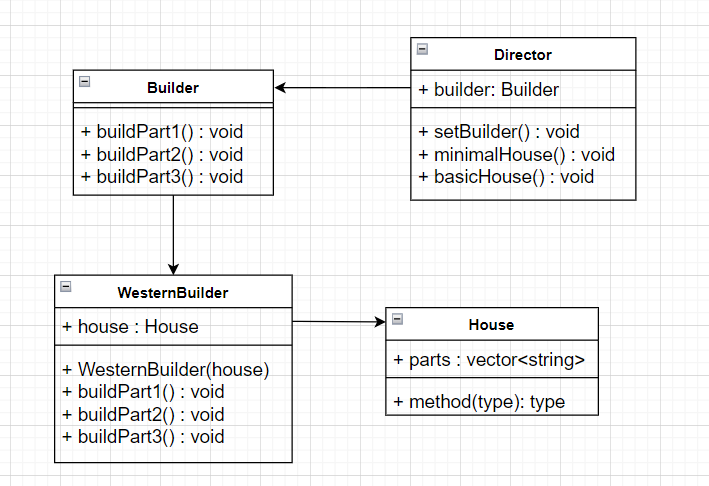
\includegraphics[scale=0.65]{image/creational/bso.png}  
\end{center}
Builder có các thành phần chính sau:
\begin{itemize}
    \item Một abstract class hay interface khai báo trước để định dạng có thể có chung cho các đối tượng sản phẩm. Người ta gọi nó là Builder.
    \item Các class kế thừa từ Builder để cung cấp cách triển khai các bước construction. Các concrete Builder này có thể được dùng để tạo ra các product không tuân theo các khuôn mẫu chung.
    \item Một class Sản phẩm là đối tượng đầu ra của kết quả được tạo nên từ Builder.
    \item Một class Director để xác địng thứ tự gọi các bước contruction.
\end{itemize}
\subsubsection{Ưu điểm và Nhược điểm }
Có thể dễ dàng thấy các ưu nhược điểm như sau:
Ưu điểm:
\begin{itemize}
    \item Builder pattern cho phép bạn xây dựng Object theo nhiều cách khác nhau bằng cách kết hợp các bước xây dựng khác nhau.
    \item Builder pattern tách biệt quy trình xây dựng Object khỏi Object cuối cùng, giúp giảm sự phức tạp của mã và tăng tính Module hóa.
\end{itemize}
Nhược điểm:
\begin{itemize}
    \item Builder pattern có thể tạo ra một lớp Builder và các bước xây dựng riêng biệt, làm tăng độ phức tạp và số lượng mã cần viết. Nếu đối tượng không phức tạp và không có nhiều tham số khác nhau, việc sử dụng Builder pattern có thể làm mã phức tạp.
\end{itemize}
\subsubsection{Code}
\begin{itemize}
    \item Ta có một căn nhà có thể được xây dựng.
    \item Đồng thời là một đội ngũ làm việc để xây dựng nên căn nhà đó. Đặc biệt là đội ngũ xây dựng nhà theo phong cách phương Tây xây nhà chia theo từng khu vực 1,2,3.
    \item Tiếp đó là một Nhà thầu chỉ định xây dựng căn nhà như thế nào.
    \item Có 2 loại nhà là loại nhà đơn giản gồm khu 1 và loại nhà căn bản gồm cả 3 khu nhà.
\end{itemize}
\begin{lstlisting}
#include <iostream>
#include <vector>
using namespace std;

class House
{
public:
    vector<string> parts;
    void show() const
    {
        cout << "House parts: ";
        for (int i = 0; i < parts.size(); i++)
            if (parts[i] == parts.back())
                cout << parts[i];
            else
                cout << parts[i] << ", ";
        cout << "\n\n";
    }
};

class Builder
{
public:
    virtual void buildPart1() = 0;
    virtual void buildPart2() = 0;
    virtual void buildPart3() = 0;
};

class WesternBuilder : public Builder
{
private:
    House *house;

public:
    WesternBuilder() { this->house = new House(); }
    void buildPart1() override { this->house->parts.push_back("Western Part1"); }
    void buildPart2() override { this->house->parts.push_back("Western Part2"); }
    void buildPart3() override { this->house->parts.push_back("Western Part3"); }

public:
    House *getResult() { return this->house; }
};

class Director
{
private:
    Builder *builder;

public:
    void setBuilder(Builder *builder) { this->builder = builder; }
    void minimalHouse() { this->builder->buildPart1(); }
    void basicHouse()
    {
        this->builder->buildPart1();
        this->builder->buildPart2();
        this->builder->buildPart3();
    }
};

int main()
{
    Director *director = new Director();
    WesternBuilder *wbuilder = new WesternBuilder();
    WesternBuilder *wbuilder1 = new WesternBuilder();
    director->setBuilder(wbuilder);
    director->minimalHouse();
    House *house = wbuilder->getResult();
    cout << "--------------minimal House 1-------------" << endl;
    house->show();
    director->setBuilder(wbuilder1);
    director->basicHouse();
    house = wbuilder1->getResult();
    cout << "--------------basic House 2-------------" << endl;
    house->show();
    return 0;
}
\end{lstlisting}
Ở hàm main, ta gọi nhà thầu, và 2 nhà xây dựng phong cách phương Tây khác nhau. Đầu tiên, nhà thầu chỉ định nhà xây dựng một xây nhà và cho ra kết quả, tiếp đó là nhà xây dựng 2 cũng tương tự.\\
\newline
\textbf{Kết quả:}
\begin{lstlisting}
--------------minimal House 1-------------
House parts: Western Part1

--------------basic House 2-------------
House parts: Western Part1, Western Part2, Western Part3    
\end{lstlisting}
\subsubsection{Các Pattern liên quan}
\begin{itemize}
    \item Có thể kết hợp với Composite do Composite cung cấp một hệ thống phân lớp phù hợp với hệ thống xây dựng nên từ các bộ phận nhỏ bằng cấp.
    \item có thể kết hợp với Iterator vì nó cung cấp khả năng duyệt qua các phần từ. Trong trường hợp này là các bước construction.
    \item Visitor cũng là một mẫu có thể được kết hợp vì nó cung cấp cách để thực hiện một hành động mới mà không ảnh hưởng đến mã nguồn của đối tượng. Trong trường hợp này có thể là có một bộ phận nhà có cách xây dựng khác với bình thường.
\end{itemize}